%
% File acl2017.tex
%
%% Based on the style files for ACL-2015, with some improvements
%%  taken from the NAACL-2016 style
%% Based on the style files for ACL-2014, which were, in turn,
%% based on ACL-2013, ACL-2012, ACL-2011, ACL-2010, ACL-IJCNLP-2009,
%% EACL-2009, IJCNLP-2008...
%% Based on the style files for EACL 2006 by 
%%e.agirre@ehu.es or Sergi.Balari@uab.es
%% and that of ACL 08 by Joakim Nivre and Noah Smith

\documentclass[11pt,a4paper]{article}
\usepackage[draft]{hyperref}
\usepackage[hyperref]{acl2017}
\usepackage{times}
\usepackage{url}
\usepackage{latexsym}
\usepackage{graphicx}
\usepackage{multirow}
\usepackage{rotating}
\usepackage{adjustbox}
\usepackage{longtable}
\usepackage{listings}
\usepackage{fancyvrb}
\usepackage{ragged2e}
\usepackage{footmisc}
\usepackage{amsmath}
\usepackage{breakcites}
\usepackage{xspace}

\newcommand{\eqnref}[1]{Equation~\ref{#1}}
\newcommand{\figref}[1]{Figure~\ref{#1}}
\newcommand{\figsref}[2]{Figures~\ref{#1} and \ref{#2}}
\newcommand{\secref}[1]{Section~\ref{#1}}
\newcommand{\secsref}[2]{Sections~\ref{#1} and \ref{#2}}
\newcommand{\sentref}[1]{(\ref{#1})}
\newcommand{\tabref}[1]{Table~\ref{#1}}
\newcommand{\tabsref}[2]{Tables~\ref{#1} and \ref{#2}}

\newcommand{\dimsum}{DiMSUM\xspace}



%\aclfinalcopy % Uncomment this line for the final submission
%\def\aclpaperid{***} %  Enter the acl Paper ID here

%\setlength\titlebox{5cm}
% You can expand the titlebox if you need extra space
% to show all the authors. Please do not make the titlebox
% smaller than 5cm (the original size); we will check this
% in the camera-ready version and ask you to change it back.

\newcommand\BibTeX{B{\sc ib}\TeX}

\title{Deep Learning Models For Multiword Expression Identification}

\author{Waseem Gharbieh \and Virendra C. Bhavsar \and Paul Cook\\
	Faculty of Computer Science, University of New Brunswick\\
	Fredericton, NB E3B 5A3 Canada\\
	{\tt \{waseem.gharbieh,bhavsar,paul.cook\}@unb.ca}}

\date{}
\aclfinalcopy

\begin{document}
\maketitle
\begin{abstract}
Multiword expressions (MWEs) are lexical items that can be decomposed
into multiple component words, but have properties that are
unpredictable with respect to their component words. In this paper we
propose the first deep learning models for token-level identification
of MWEs. Specifically, we consider a layered feedforward network, a
recurrent neural network, and convolutional neural networks. In
experimental results we show that convolutional neural networks are
able to outperform the previous state-of-the-art for MWE
identification, with a convolutional neural network with three hidden
layers giving the best performance.
\end{abstract}

\section{Introduction}

%% Human language contains ambiguities on multiple levels, from the
%% simple words that we use in a literal manner every day to the
%% idiosyncratic expressions whose meaning cannot be inferred from the
%% words making up those expressions. In linguistics, these idiosyncratic
%% expressions are called multiword expressions (MWEs). They combine
%% words in various ways to produce phrases that have properties that are
%% not predictable from the properties of their individual words or their
%% normal mode of combination. This includes proverbs such as \textit{Two
%%   wrongs don't make a right}, proper names or named entities, for
%% example \textit{Prime Minister Justin Trudeau}, and verb noun
%% combinations as in \textit{hit the roof} or \textit{blow the whistle},
%% among many other classes which motivated some linguists to call them a
%% ``pain in the neck" for Natural Language Processing (NLP)
%% \cite{sag2002multiword}. Identifying these expressions can have a
%% significant impact on many NLP tasks such as machine translation
%% \cite{carpuat2010task}, information retrieval
%% \cite{newman2012bayesian} and opinion mining
%% \cite{berend2011opinion}. An in-depth discussion about integrating
%% MWEs into NLP tasks is presented in section \ref{MWEID}.



Multiword expressions (MWEs) are lexical items that can be decomposed
into multiple component words, but have properties that are idiomatic,
i.e., marked or unpredictable, with respect to properties of their
component words \cite{Baldwin:Kim:2010}. MWEs include a wide range of
phenomena such as noun compounds (e.g., \textit{speed limit} and
\textit{monkey business}), verb--particle constructions (e.g.,
\emph{clean up} and \emph{throw out}), and verb--noun idiomatic
combinations (e.g., \textit{hit the roof} and \textit{blow the
  whistle}), as well as named entities (e.g., \textit{Prime Minister
  Justin Trudeau}) and proverbs (e.g., \textit{Two wrongs don't make a
  right}). One particular challenge for natural language processing
(NLP) is MWE identification --- i.e., to identify which tokens in
running text correspond to MWEs so that they can be analyzed
accordingly. The challenges posed by MWEs have led to them to be
referred to as a ``pain in the neck'' for NLP \cite{sag2002multiword};
nevertheless, incorporating knowledge of MWEs into NLP applications
can lead to improvements in tasks including machine translation
\cite{carpuat2010task}, information retrieval
\cite{newman2012bayesian}, and opinion mining
\cite{berend2011opinion}.

Recent work on token-level MWE identification has focused on methods
that are applicable to the full spectrum of kinds of MWEs
\cite{schneider2014discriminative}, in contrast to earlier work that
tended to focus on specific kinds of MWEs
\cite{Uchiyama2005,Fazly2009,Fothergill:Baldwin:2012}. Deep learning
is an emerging class of machine learning models that have recently
achieved promising results on a range of NLP tasks such as machine
translation \cite{bahdanau2014neural,sutskever2014sequence}, named entity recognition \cite{DBLP:conf/naacl/LampleBSKD16}, natural
language generation \cite{DBLP:conf/acl/LiLJ15}, and sentence
classification \cite{DBLP:conf/emnlp/Kim14}. Such models have,
however, not yet been applied to broad-coverage MWE identification.

In this paper we propose the first deep learning models for
broad-coverage MWE identification. Specifically, we propose and
evaluate a layered feedforward network, a recurrent neural network,
and two convolutional neural networks. We compare these models against
the previous state-of-the-art \cite{DBLP:conf/semeval/KirilinKV16} and
several more-traditional supervised machine learning approaches. We
show that the convolutional neural networks outperform the previous
state-of-the-art. This finding is particularly remarkable given the
relatively small size of the training data available, and demonstrates
that deep learning models are able to learn well from small
datasets. Moreover, we show that our proposed deep learning models are
able to generalize more-effectively than previous approaches, based on
comparisons between the models' performances on validation and test
data.



%% Generalization



%% In this paper, our aim is to examine the performance of an emerging
%% class of machine learning models called deep learning models, for
%% identifying MWEs in running text. Their performance is then compared
%% to traditional machine learning models and current MWE identification
%% systems.

%% Our objectives are to answer the following research questions:

%% 1) Are deep learning models able to beat the state-of-the-art system
%% for MWE identification?

%% For this research question, we will be comparing the F-scores achieved
%% by our deep learning models with the current state-of-the-art F-score
%% \cite{DBLP:conf/semeval/KirilinKV16}.

%% 2) Do deep learning models generalize effectively?

%% Here, we compare the performance of the models on the validation set
%% with their performance on the test set. A model is said to generalize
%% well if its performance on the test set closely matches its
%% performance on the validation set. To generalize effectively, the
%% ratio of the performance of the model on the test set to its
%% performance on the validation set should be greater than the ratio of
%% the model proposed by \cite{schneider2014discriminative} which was the
%% first model for tackling MWE identification.

%% 3) Do deep learning models perform well on small datasets?

%% The data set used to train the deep learning models for this task is
%% relatively small compared to the typical data sets used to train deep
%% learning models. One of the ways in which this problem can be
%% alleviated is by using distributed representations of tokens learned
%% from Wikipedia as part of the input features.

%% This paper has three main contributions. First, we propose and
%% evaluate the performance of a Layered Feedforward Network, a
%% recurrent neural network, and two convolutional neural
%% networks. Second, the results show that the fully connected neural
%% network and the two convolutional neural networks are able to perform
%% well on this task even with the limited amount of data
%% available. Third, we achieve more than 1\% F-score improvement over
%% state-of-the-art performance on the MWE identification task. Last but
%% not the least, this is the first work that applies deep learning
%% models for broad MWE identification.

\section{Related Work} \label{MWEID}

%% MWE identification is defined as the detection of literal and MWE
%% usages of word combinations.

%A large amount of work has been done in NLP on MWE identification as
%well as various other MWE tasks such as: extraction, compositionality
%prediction, and incorporating MWEs into other NLP applications. MWE
%extraction is a token level task where given a corpus, we want to
%generate an MWE lexicon. It can be said that MWE identification
%tackles MWE extraction but not the other way around. Compositionality
%prediction detects whether the meaning of an MWE is determined by the
%meanings of its constituent expressions. The task has been approached
%using statistical methods such as measuring the distributional
%similarity of the extracted features
%\cite{korkontzelos2009detecting}, or vector space models
%\cite{katz2006automatic,kiela2013detecting,DBLP:conf/mwe/KrcmarJP13}
%and more recently, by using distributed word representations
%\cite{DBLP:conf/naacl/SalehiCB15}. Since MWEs compose a sizable
%amount of an individual’s vocabulary, incorporating MWEs into other
%applications can help improve their
%performance. \cite{jackendoff1997architecture} estimated that the
%number of MWEs used by an individual is of the same order of
%magnitude as the number of words in their vocabulary and new MWEs are
%being invented all the time. \cite{carpuat2010task} demonstrated that
%a machine translation system obtained a 0.78 point increase in its
%BLEU score after incorporating the WordNet MWE lexicon compared to
%the baseline machine translation
%system. \cite{finlayson2011detecting} reported that using a
%straight-forward MWE detection strategy led to an absolute 5\%
%improvement in Word Sense Disambiguation (WSD) F-score while perfect
%MWE detection led to an absolute 6.1\% improvement in WSD
%F-score. \cite{constant2011mwu} was able to obtain a state-of-the-art
%French POS tagger by including features from external MWE
%lexicons. In addition, their model achieved 91\% precision and 71\%
%recall for detecting French MWEs.

MWE identification is the task of determining, at the token level,
which words are parts of MWEs, and which are not. For example, in the
sentence \emph{The staff leaves a lot to be desired} (also used in
\figref{fscore}) \emph{a lot} and \emph{leaves
  \underline{\phantom{xxx}} to be desired} are MWEs. An important part
of MWE identification is to be able to distinguish between MWEs and
literal combinations that have the same surface form; e.g., \emph{kick
  the bucket} is ambiguous between an idiomatic usage --- meaning
roughly `die' --- which is an MWE, and a literal one which is
not. Many earlier studies on MWE identification have focused on this
type of ambiguity, and treated the problem as one of word sense
disambiguation, where literal and idiomatic usages are considered
different word senses \cite{Birke2006,Katz2006,Li+:2010}. Other work
has leveraged linguistic knowledge of properties of MWEs in order to
make these distinctions
\cite{Uchiyama2005,Fazly2009,Fothergill:Baldwin:2012}. Crucially, this
work has typically focused on specific kinds of MWEs, and has not
considered identification of the full spectrum of MWEs.


%% Early work on MWE identification mainly consisted of approaches based
%% on statistical measures of extracted features
%% \cite{ramisch2008evaluation} or feeding these measures to a machine
%% learning algorithm \cite{pecina2008machine,ramisch2010mwetoolkit}.A
%% more recent semi-supervised approach was also proposed
%% \cite{DBLP:conf/mwe/RondonCR15} using the never-ending learning
%% approach by \cite{DBLP:conf/aaai/MitchellCHTBCMG15}.  Their system
%% collected textual data from the web to build a corpus. The corpus was
%% then annotated with their surface form, POS tag and lemma. The
%% mwetoolkit \cite{ramisch2010mwetoolkit} was then used to calculate
%% some association measures. These association measures were then
%% combined with other features such as the POS context surrounding the
%% MWE as well as a translatability feature (which measures the
%% probability of an adjective or noun to be translated to a word in
%% English and back to Portuguese) and fed to an SVM.


%% Schneider et al. overview


%% The first attempt to evaluate the effectiveness of broad MWE
%% identifiers on a sizable corpus was done by
%% \cite{schneider2014discriminative}. It proposed a supervised learning
%% model based on the structured perceptron
%% \cite{collins2002discriminative} for identifying all classes of
%% MWEs. The system was built for general-purpose MWE identification
%% using the BIO convention where B indicates the beginning of an MWE, I
%% indicates the continuation of an MWE, and O indicates that the token
%% is not part of an MWE. The features of the model contain a group of
%% basic features such as POS tags and lists of MWEs that have been taken
%% from multiple lexicons such as WordNet, SemCor, and WikiMwe. The
%% authors also make use of unsupervised Brown clusters, which clusters
%% tokens based on their contextual similarity
%% \cite{DBLP:journals/coling/BrownPdLM92} and compare their supervised
%% approach to a baseline that classifies a sequence of tokens as MWEs if
%% they are present in the lexicons. Their results on the MWE corpus
%% \cite{schneider2014comprehensive} revealed that using the supervised
%% model with oracle POS and brown clusters along with a penalty for
%% higher recall, achieves the best exact match
%% F-scores. \cite{qu2015big} later improved upon that system by using
%% skip-gram instead of Brown clusters with a variant of Conditional
%% Random Fields (CRFs).


%% The approach involved three major steps: extraction of common
%% $n$-grams, initial segmentation, and refinement of the resulting
%% lexicon. The text was preprocessed by setting a maximum value of $n$
%% for the $n$-grams to be extracted. Then $n$-grams were segmented
%% depending on the predictability of the sequence. Lastly, the resulting
%% lexicon was refined by splitting each segmentation containing more
%% than 3 tokens even further if the difference between the
%% predictability of the tokens in the current segmentation and the
%% predictability of the new segmentation by itself was less than the log
%% of the ratio between the counts of the new segmentation and the counts
%% of the current segmentation.

%% An unsupervised learning approach was presented by
%% \cite{DBLP:conf/coling/BrookeTHS14}. The main idea is to segment the
%% corpus into multiword units. The approach involved three major steps:
%% Extraction of common n-grams, initial segmentation, and refinement of
%% the resulting lexicon. The text was preprocessed by setting a maximum
%% value of $n$ for the n-grams to be extracted. Then it was segmented
%% depending on the predictability of the sequence. Lastly, the resulting
%% lexicon was refined by splitting each segmentation containing more
%% than 3 tokens even further if the difference between the
%% predictability of the tokens in the current segmentation and the
%% predictability of the new segmentation by itself is less than the log
%% of the ratio between the counts of the new segmentation and the counts
%% of the current segmentation.



More-recent work has considered the identification of a wider range of
types of MWEs. \newcite{DBLP:conf/coling/BrookeTHS14} present an
unsupervised learning approach to segment a corpus into multiword
units based on their predictability.
\newcite{schneider2014discriminative} propose methods for
broad-coverage MWE identification, and evaluate them on a sizeable
corpus \cite{schneider2014comprehensive}. They proposed a supervised
learning approach based on the structured perceptron
\cite{collins2002discriminative}. The system labels tokens using the
     {\fontfamily{lmtt}\selectfont BIO} convention, where
     {\fontfamily{lmtt}\selectfont B} indicates the beginning of an
     MWE, {\fontfamily{lmtt}\selectfont I} indicates the continuation
     of an MWE, and {\fontfamily{lmtt}\selectfont O} indicates that
     the token is not part of an MWE. The model includes features
     based on part-of-speech tags, MWE lexicons, and Brown clusters
     \cite{DBLP:journals/coling/BrownPdLM92}.  \newcite{qu2015big}
     later improved upon that system by using skip-gram embeddings
     \cite{mikolov2013distributed} instead of Brown clusters with a
     variant of conditional random fields. More recently,
     \newcite{DBLP:conf/acl/ConstantN16} incorporate MWE
     identification along with dependency parsing by forming two
     representations for a sentence: a tree that represents the
     syntactic dependencies, and a forest of lexical trees that
     includes the MWEs identified in the sentence.


%% \cite{DBLP:conf/acl/ConstantN16} presented another approach for
%% identifying regular and irregular MWEs without compromising the
%% syntactic representation.  The main idea is to produce two
%% representations: One is a tree that represents the syntactic
%% dependencies and another is a forest of lexical trees that includes
%% the MWEs identified in the sentence. These representations were formed
%% using a transition-based model and a linear model was trained to score
%% the transition sequences.  A greedy search algorithm was then used to
%% find the highest scoring transition.



%% Discuss SemEval shared task and Kirilin work 

%% Recently, a Semeval task was announced for Detecting Minimal Semantic
%% Units and their Meanings (DiMSUM). The aim of the task was to come up
%% with an MWE identification and Supersense tagging models
%% \cite{DBLP:conf/semeval/SchneiderHJC16}. To evaluate the performance
%% of the submitted models, a larger corpus was composed from multiple
%% corpora. 6 teams participated in this task with 5 teams publishing
%% their approaches. The winning team, ICL-HD
%% \cite{DBLP:conf/semeval/KirilinKV16} took into consideration all of
%% the basic features used by \cite{schneider2014discriminative} and two
%% other feature sets. The first one is based on the YAGO anthology where
%% some heuristics were applied for potential named entities to extract
%% them from the anthology. The second feature set was GloVe
%% \cite{Pennington+:2014} with the word vectors scaled by a constant and
%% divided by the standard deviation of each of its dimensions. The 
%% experiments revealed that adding the YAGO features (and combining
%% WordNet hypernyms as well as supersense ranking) improved MWE
%% detection by 0.59 and SST by 1.13. It was also found that scaling the
%% GloVe vectors by 1 (no scaling) was best for the SST and combined task
%% but scaling them by 0.01 was more appropriate for the MWE detection
%% task. That being said, combining YAGO and GloVe did not improve upon
%% the performance of GloVe.

The recent SemEval shared task on Detecting Minimal Semantic Units and
their Meanings (DiMSUM) focused on MWE identification along with
supersense tagging \cite{DBLP:conf/semeval/SchneiderHJC16}. The best
performing system for MWE identification for this shared task was that of
\newcite{DBLP:conf/semeval/KirilinKV16} which took into consideration all of
the basic features used by \newcite{schneider2014discriminative} and
two
%% CPC: Waseem: Add a citation for YAGO anthology
novel feature sets. The first one is based on the YAGO ontology \cite{DBLP:conf/www/SuchanekKW07},
where heuristics were applied to extract potential named entities from the ontology. The second feature set was GloVe
\cite{Pennington+:2014} word embeddings, with the word vectors scaled
by a constant and divided by the standard deviation of each of its
dimensions. None of the systems that participated in the DiMSUM shared
task considered deep learning approaches.

In this paper we propose the first deep learning approaches to MWE
identification. We use the DiMSUM data for training and evaluating our
models, and compare against the state-of-the-art method of
\newcite{DBLP:conf/semeval/KirilinKV16}. Here we focus solely on
the MWE identification task, leaving supersense tagging for future
work.




%% The experiments revealed that adding the YAGO features (and combining
%% WordNet hypernyms as well as supersense ranking) improved MWE
%% detection by 0.59 and SST by 1.13. It was also found that scaling the
%% GloVe vectors by 1 (no scaling) was best for the SST and combined task
%% but scaling them by 0.01 was more appropriate for the MWE detection
%% task. That being said, combining YAGO and GloVe did not improve upon
%% the performance of GloVe.

%% . The aim of the task was to come up with an MWE identification and
%% Supersense tagging models \cite{DBLP:conf/semeval/SchneiderHJC16}. To
%% evaluate the performance of the submitted models, a larger corpus was
%% composed from multiple corpora. 6 teams participated in this task with
%% 5 teams publishing their approaches.


%% The winning team, ICL-HD \cite{DBLP:conf/semeval/KirilinKV16} took
%% into consideration all of the basic features used by
%% \cite{schneider2014discriminative} and two other feature sets. The
%% first one is based on the YAGO anthology where some heuristics were
%% applied for potential named entities to extract them from the
%% anthology. The second feature set was GloVe \cite{Pennington+:2014}
%% with the word vectors scaled by a constant and divided by the standard
%% deviation of each of its dimensions. The experiments revealed that
%% adding the YAGO features (and combining WordNet hypernyms as well as
%% supersense ranking) improved MWE detection by 0.59 and SST by 1.13. It
%% was also found that scaling the GloVe vectors by 1 (no scaling) was
%% best for the SST and combined task but scaling them by 0.01 was more
%% appropriate for the MWE detection task. That being said, combining
%% YAGO and GloVe did not improve upon the performance of GloVe.




%% Remove this discussion and just say that none of the other approaches
%% use deep learning... use this to position our work with respect to
%% what's come before... Emphasize that we focus on only the MWE id bit...


%% Other approaches for tackling this task included using a
%% double-chained CRF to separate the labelling of MWEs and supersenses
%% and used the Viterbi algorithm to produce the sequence with the
%% highest probability
%% \cite{DBLP:conf/semeval/HosseiniSL16}. \cite{DBLP:conf/semeval/CordeiroRV16}
%% used a rule-based approach and extracted type features using the
%% mwetoolkit and discarded the MWE candidates that occurred less than a
%% threshold value. \cite{DBLP:conf/semeval/ScherbakovV0B16} utilized 300
%% dimensional CBOW word embeddings for known words and a hash function
%% for unknown words and various word features. The MWEs were detected by
%% first iterating through the input sentence and choosing the head word
%% of the MWE, after that, another loop was executed through the
%% remaining words to determine whether they were a part of that MWE or
%% not. \cite{DBLP:conf/semeval/BjorneS16} detected MWEs using dictionary
%% matching. The authors also used the Yelp and Wikipedia taggers to
%% identify nouns and names. For each token, the lemma, POS, and word
%% values were included and for the first and last tokens in the set, the
%% positions of the tokens were also supplied and fed to an Extra trees
%% classifier.








\section{Neural Network Models}

%% Therefore, the input features had a value of 0
%% most of the time. 


In this section, we discuss the features extracted for the neural
network models, and the model
architectures. \newcite{schneider2014comprehensive} extracted roughly
320k sparse features. Because of the large input feature space, the
only feasible way to train a model on those features is by using a
linear classifier.  In contrast to
\newcite{schneider2014comprehensive} our aim is to create dense input
features to allow neural network architectures, as well as other
machine learning algorithms, to be trained on them. Specifically, we
propose three neural network models: a layered feedforward network
(LFN), a recurrent neural network (RNN), and a convolutional neural
network (CNN).\footnote{In preliminary experiments we also considered
  a sequence-to-sequence model \cite{DBLP:conf/emnlp/ChoMGBBSB14}, but found it to
  perform poorly relative to the other models, and so do not discuss
  it further.}


%% Furthermore, some of the features included suggest
%% a substantial amount of feature engineering was carried out by the
%% authors, for example, a binary feature that indicates whether the
%% target token has the same POS tag as a token in its context.
%% Added to that, there was a lot of feature engineering involved by the
%% authors. This is evident in some of the features that they provide to
%% the model such as, a binary feature that indicates whether the target
%% token occurs with a context POS, another binary feature that indicates
%% whether the context tokens occur with the target token's POS, the
%% lemma and context lemma if one of them is a verb and the other is a
%% noun, verb, adjective, adverb, preposition, or particle, and most of
%% the 8 types of features extracted from the lexicons.



\subsection{Layered Feedforward Network} \label{LFN1}

Although LFNs have been used to solve a wide range of classification
and regression problems, they have been shown to be less effective for
tasks at which deep learning models excel, such as image
classification \cite{DBLP:conf/nips/KrizhevskySH12} and machine
translation \cite{bahdanau2014neural}. The LFN is therefore proposed
as a benchmark for comparing the performance of the other
architectures, as well as for developing informative input
features. Most feature engineering was carried out while developing
this model and then transferred to the other architectures.

The composition of the \dimsum corpus
\cite{DBLP:conf/semeval/SchneiderHJC16}, and the token-level lemma and
part-of-speech annotations it provides, influenced our feature
extraction. Most of the text in the \dimsum corpus is social media
text. The tokens and lemmas were therefore preprocessed by removing
\emph{\#} characters from tokens and lemmas that contain them, and
mapping URLs, numbers, and any token or lemma containing the \emph{@}
symbol to the special tokens \emph{URL}, \emph{NUMBER}, and
\emph{USER}, respectively. After pre-processing, distributed
representations of all tokens and lemmas were obtained from a
skip-gram \cite{mikolov2013distributed} model.  Specifically, the
gensim \cite{rehurek_lrec} implementation of skip-gram was trained on
a snapshot of Wikipedia from September 2015 to learn 100 dimensional
word embeddings. Any token occurring less than 15 times was discarded,
the context window was set to 5, the negative sampling rate was set to
5, and unknown tokens were represented with a zero vector. The
part-of-speech tag for each token was also encoded, in this case as a
one-hot vector.



%% The Skip-gram model was used to obtain the distributed
%% representations of the tokens and lemmas. The Skip-gram model is one
%% of the two word2vec models proposed by \cite{mikolov2013distributed}
%% that learns distributed representations of word meaning in the form of
%% word embeddings by predicting the context of a given target type. 

%% To obtain reliable word representations, the Skip-gram model was
%% trained on a September 2015 snapshot of Wikipedia to learn 100
%% dimensional word embeddings using a library called gensim. Any token
%% occurring less than 15 times was discarded, the context window was set
%% to 5, the negative sampling rate was set to 5, and unknown tokens
%% where represented with a zero vector. For POS tags, one hot vector
%% encoding was used to indicate which POS tag the respective token and
%% lemma belonged to.



%% Looking at some of the features employed by
%% \cite{schneider2014discriminative}, we saw that using word shape
%% features can help MWE identification. 

\newcite{schneider2014discriminative} included word shape features,
which can be informative for the identification of MWEs, especially
named entities. We therefore also include word shape features. These
are binary features for each token and lemma that capture whether it
includes single or double quotes; consists of all capital letters;
starts with a capital letter (but is otherwise lowercase); contains a
number; includes a \emph{\#} or \emph{@} character; corresponds to a
URL; contains any punctuation; and consists entirely of punctuation
characters.

%% Therefore, we used separate

%% binary features for the tokens and lemmas to 

%% indicate the presence of single and double quotes, 

%% whether they were entirely made up of capital letters,

%% if they started with a capital letter (but were otherwise lowercase),

%% whether they contained a number, 

%% if they consisted entirely of numbers, 

%% if the token or lemma had a `\#' or `@' in it, 

%% and whether they were a URL, 

%% if they contained punctuation, and

%% whether they were punctuation. 

\newcite{schneider2014discriminative} include features based on MWE
lexicons that represent which tokens and lemmas are potentially part
of an MWE and according to which lexicon. We use a script provided by
\newcite{schneider2014discriminative} to include these same features
in our representation.


%% also had a script that analyzed
%% the MWEs in a sentence based on MWE lexicons. We used this script to
%% analyze which tokens and lemmas were potentially part of an MWE and
%% which lexicon lead to that conclusion.

Finally, \newcite{DBLP:conf/acl/SaltonRK16} showed that embedding the
entire sentence in which a target MWE occurs was helpful for
distinguishing idiomatic from literal verb--noun idiomatic
combinations. We therefore also include a representation for the
entire sentence. Specifically, we separately average the skip-gram
embeddings for the tokens and lemmas in the sentence containing the
target word. These features were then input into an LFN model with a
single hidden layer, which we refer to as LFN1.


\subsection{Recurrent Neural Network\label{sec:rnn}}

RNNs are a natural fit for many NLP problems due to their ability to
model sequences. Here we apply an RNN to broad coverage MWE
identification. The token for the current time step is represented
using the same features as LFN1 described above, except we do not
include the average of the skip-gram representations for tokens and
lemmas in the same sentence as the target word because we expect the
RNN to be able to learn a representation of the sentence by itself. We
use a single layer RNN model, referred to as RNN1.


%% To put this ability to the test, all the LFN features for the token
%% at the current timestep were taken. Therefore, the Skip-gram
%% representation of the target token as well as its lemma was extracted
%% after preprocessing. In addition, its POS tag as well as the analysis
%% whether the token and its lemma were potentially a part of an MWE was
%% obtained. The average of the token and lemma Skip-gram representations
%% was not provided as the RNN is expected to learn this representation
%% by itself. A single layer RNN model (RNN1) was examined from this
%% family of models.

\subsection{Convolutional Neural Network}
CNNs have been shown to be powerful classifiers
\cite{DBLP:conf/emnlp/Kim14,DBLP:conf/aaai/KimJSR16}, and since MWE
identification can be formulated as a classification task, CNNs have
the potential to perform well on it. The feature representation for
the CNN was split into feature columns to enable the implementation of
the convolution layer. Each feature column contains the same features
as those for the RNN at each time step but since the CNN does not
learn sequential information, a window of feature columns was given as
an input.

Multiple filters can then be applied on these feature columns to
extract different local features across different window sizes. After
finding the optimal number of filters and their sizes, a max-pooling
operation is executed on the values extracted by the feature map to
form the hidden layer which will be used to produce the predicted
output. For our evaluation, we use CNN architectures with two and
three fully connected hidden layers, which we refer to as CNN2 and CNN3, respectively. We observed that CNNs with 2 and 3 hidden layers performed well on the validation set but adding more layers resulted in overfitting. Similarly, adding more hidden layers to the LFN and RNN also resulted in overfitting. 



%% CPC: Waseem: Justify here why you consider 2 and 3 hidden layers for
%% the CNN while for the LFN and RNN you only consider 1 hidden layer.

\section{Data and Evaluation}

This section presents the statistics and structure of the dataset used
for this task, as well as the evaluation methodology.

\subsection{Dataset}

We use the DiMSUM dataset \cite{DBLP:conf/semeval/SchneiderHJC16} for
our experiments, which allows for direct comparison with previous
results.
%% The dataset used for this task is the dataset that was released for
%% the DiMSUM task mentioned in section \ref{MWEID}. 
Table \ref{dataset_stats} displays the source corpora from which the
dataset was constructed; their domain (i.e., reviews, tweets, or TED
talks); the number of sentences, words, MWEs, and gappy (i.e.,
discontiguous) MWES in each source corpus; and the percentage of
tokens belonging to an MWE in each source corpus. The dataset is split
into training and testing sets such that the testing data contains a
novel text type, i.e., TED talks. 

For parameter tuning purposes, we also require validation data. We
form a validation set from the training data by splitting the training
data to create 5 folds, where every fold contained 20\% validation
data, and the remaining 80\% was used for training.


%% In our case, the training portion was further split to create 5
%% folds, where every fold contained 80\% training data and 20\%
%% validation data; this validation data was used to tune model
%% parameters.

%\begin{turn}{90}\textbf{Train}\end{turn}

\begin{table*}
	\begin{center}
		%\textwidth
		%\columnwidth
		\resizebox{\textwidth}{!}{%
			\begin{tabular}{cccccccc}
				
				\textbf{Split} & \textbf{Domain} & \textbf{Source corpus} & \textbf{Sentences} & \textbf{Words} & \textbf{MWEs} & \textbf{Gappy MWEs} & \textbf{\% tokens in MWE} \\ \hline
				\multirow{3}{*}{\textbf{Train}} & REVIEWS & STREUSLE 2.1 {\scriptsize \cite{schneider2015corpus}} & 3,812 & 55,579 & 3,117 & 397 & 13\%\\
				& TWEETS & Lowlands {\scriptsize \cite{DBLP:conf/starsem/JohannsenHAPS14}} & 200 & 3,062 & 276 & 5 & 22\%\\
				& TWEETS & Ritter {\scriptsize \cite{DBLP:conf/emnlp/RitterCME11,DBLP:conf/starsem/JohannsenHAPS14}} & 787 & 15,185 & 839 & 65 & 13\%\\ \hline
				& & \textbf{Train Total} & 4,799 & 73,826 & 4,232 & 467 & 13\% \\ \hline
				\multirow{4}{*}{\textbf{Test}} & REVIEWS & Trustpilot {\scriptsize \cite{DBLP:conf/www/HovyJS15}} & 340 & 6,357 & 327 & 13 & 12\%\\
				& TWEETS & Tweebank {\scriptsize \cite{DBLP:conf/emnlp/KongSSBDS14}} & 500 & 6,627 & 362 & 20 & 13\% \\
				& TED & NAIST-NTT {\scriptsize \cite{cettolo2012web,neubig2014the}} & 100 & 2,187 & 93 & 2 & 9\%\\ 
				& TED & IWSLT test {\scriptsize \cite{cettolo2012web}} & 60 & 1,329 & 55 & 1 & 9\%\\\hline
				& & \textbf{Test Total} & 1,000 & 16,500 & 837 & 36 & 12\% \\ \hline
				%% & & \textbf{REVIEWS Total} & 4,152 & 61,936 & 3,444 & 410 & 13\% \\
				%% & & \textbf{TWEETS Total} & 1,487 & 24,874 & 1,477 & 90 & 14\% \\
				%% & & \textbf{TED Total} & 160 & 3,516 & 148 & 3 & 9\% \\ \hline
				%% & & \textbf{Grand Total} & 5,799 & 90,326 & 5,069 & 503 & 13\% \\
				
		\end{tabular}}
		\caption{Statistics describing the composition of the
			\dimsum dataset.}
		\label{dataset_stats}
	\end{center}
\end{table*}

\subsection{Structure}

Every line in the dataset provides 8 pieces of information: the
numeric position of the token in its sentence; the token itself; its
lemmatized form; its part-of-speech tag; its gold-standard MWE tag;
the position of the last token that is part of its MWE; its supersense
tag;\footnote{\newcite{schneider2014discriminative} consider MWE
  identification and super-sense tagging. We focus only on MWE
  identification in this work and so don't use the super-sense tag
  information provided in the dataset.} and the sentence ID. Six MWE
tags are used for MWE identification in this dataset,
{\fontfamily{lmtt}\selectfont B} which indicates the beginning of an
MWE, {\fontfamily{lmtt}\selectfont I} which indicates the continuation
of an MWE, {\fontfamily{lmtt}\selectfont O} which indicates that the
token is not part of an MWE, {\fontfamily{lmtt}\selectfont b}
indicates the beginning of a new MWE inside an MWE,
{\fontfamily{lmtt}\selectfont i} indicates the continuation of the new
MWE inside an MWE, and finally, {\fontfamily{lmtt}\selectfont o}
indicates that the token that is inside an MWE is not part of the
nested MWE. This convention assumes that MWEs can only be nested to a
depth of one (i.e., an MWE inside an MWE), and that MWEs must be
properly nested.

\subsection{Performance Metric}

We use the link-based F-score evaluation metric from
\newcite{schneider2014discriminative}, which allows for direct
comparison with prior work. \tabref{dataset_stats} shows that the
percentage of tokens occurring in MWEs ranges from 9--22\%. As such,
MWEs occur much less frequently than literal word combinations.  This
evaluation metric correspondingly puts more emphasis on the ability of
the model to detect MWEs rather than literal word combinations.

\begin{figure}
	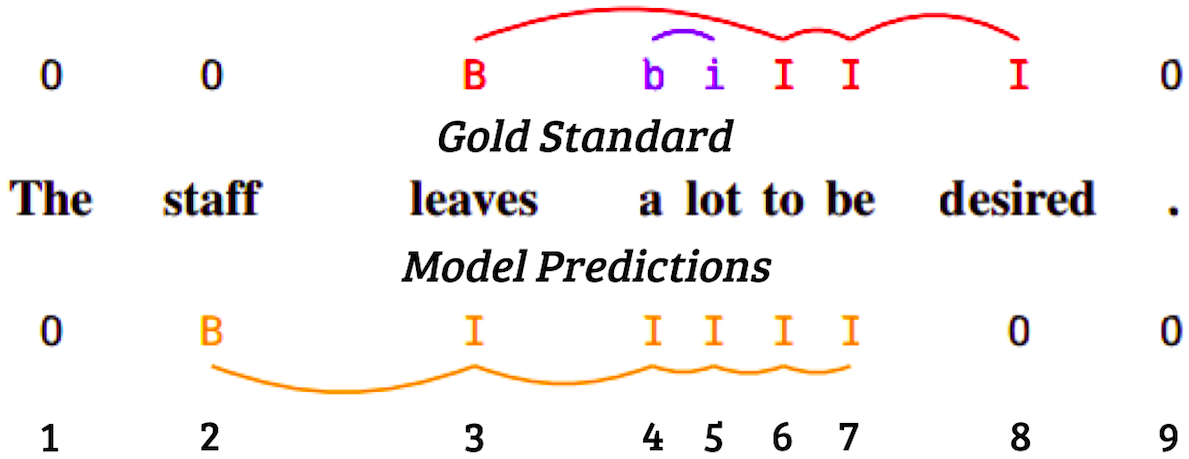
\includegraphics[width=\linewidth]{AugFscore2.png}
	\caption{An example of how a model could tag a sequence, along
		with its gold standard tagging (adapted from
		\newcite{DBLP:conf/semeval/SchneiderHJC16}).}
	\label{fscore}
\end{figure}

Figure \ref{fscore} is a diagram adapted from
\newcite{DBLP:conf/semeval/SchneiderHJC16} which shows an example of
how a model could tag a sequence, as well as its gold standard
tagging.  The MWE tags on top represent the gold standard, and the MWE
tags predicted by a system are shown on the bottom. A link is defined
as the path from one token to another, as in \figref{fscore},
regardless of the number of tokens in that path. Precision is
calculated as the ratio of the number of correctly predicted links to
the total number of links predicted by the model. Recall is calculated
in the same way but swapping the gold standard and predicted links.

For example, in \figref{fscore}, the model was able to correctly
predict two links.  The first link goes from
{\fontfamily{lmtt}\selectfont b} to {\fontfamily{lmtt}\selectfont i}
in the gold standard which is matched by a predicted link from token
4--5 by the model. The second link is from token 6--7 in the gold
standard which matches the model's prediction. Since the model
predicted five links in total, the precision is $\frac{2}{5}$.

To calculate recall, the roles of the gold standard and model
predictions are reversed. This way, three links have been correctly
predicted. Two of the three links are the previously mentioned
links. The third one is the link from {\fontfamily{lmtt}\selectfont B}
to {\fontfamily{lmtt}\selectfont I} in the gold standard which
corresponds to the path from token 3--6. Because there are four links
in the gold standard, the recall is therefore $\frac{3}{4}$.

The F-score is then calculated based on precision and recall according
to the following equation:

\begin{equation}
\frac{1}{F} = \frac{1}{2} (\frac{1}{P} + \frac{1}{R})
\end{equation}
\vspace{5mm}

\noindent
where $F$ is the F-score, and $P$ and $R$ are precision and recall,
respectively.


%% Figure \ref{fscore} is a diagram adapted from
%% \cite{DBLP:conf/semeval/SchneiderHJC16} which shows an example of how
%% a model could tag a sequence as well as its gold standard. Assuming
%% that the MWE tags at the top are the gold standard, and that the
%% predicted MWE tags are at the bottom, the model was able to correctly
%% predict 2 links.  The first link goes from
%% {\fontfamily{lmtt}\selectfont b} to {\fontfamily{lmtt}\selectfont i}
%% in the gold standard which is matched by a predicted link from the
%% fourth token to the fifth one by the model. The second link is from
%% the sixth token to the seventh token in the gold standard which
%% matches the model's prediction. Since the model predicted 5 links in
%% total, the precision is $\dfrac{2}{5}$.

%% To calculate recall, the roles of the gold standard and model
%% predictions are reversed. This way, 3 links have been correctly
%% predicted. Two of the three links are the previously mentioned
%% links. The third one is the link from {\fontfamily{lmtt}\selectfont B}
%% to {\fontfamily{lmtt}\selectfont I} in the gold standard which
%% corresponds to the path from the third token to the sixth. Following
%% the same logic as in the precision calculation, since there are 4
%% links in the gold standard, the recall is $\dfrac{3}{4}$ which gives
%% an F-score of $\dfrac{12}{23}$.

\section{Parameter Settings}

In this section, the architecture and parameters of all neural network
models are presented in detail. The cost function used to train the
neural network models was based on the cost function used by
\newcite{schneider2014discriminative} for this task:

\begin{equation}
cost = \sum_{i=1}^{|\bar{y_i}|} c(\bar{y_i},y_i) 
\label{eqn:cost}
\end{equation} 

\vspace{5mm}

\noindent
where $\bar{y_i}$ is the $i$th gold standard MWE tag, and $y_i$ is the
$i$th MWE tag predicted by the neural network model. To ensure that
the MWE tag predicted by the neural network is a probability
distribution, the output layer of all neural models was the softmax
layer. The function $c$ in \eqnref{eqn:cost} is defined as:

\begin{equation}
c(\bar{y_i},y_i) = \bar{y_i} \log(y_i) + \rho (\bar{y_i} \epsilon \{B\} \land y_i \epsilon \{O\})
\label{eqn:c}
\end{equation}

\vspace{5mm}


Some MWE tag sequences are invalid, for example, a
{\fontfamily{lmtt}\selectfont B} followed immediately by an
{\fontfamily{lmtt}\selectfont O} (because MWEs are composed of
multiple tokens), and similarly, an {\fontfamily{lmtt}\selectfont O}
cannot occur immediately before an {\fontfamily{lmtt}\selectfont I}
(because the beginning of every MWE must be tagged with a
{\fontfamily{lmtt}\selectfont B}).  We therefore use the Viterbi
algorithm on the output of the neural network models to obtain the
valid MWE tag sequence with the highest probability. In preliminary
experiments we observed that setting all valid transitions to be of
equal probability, and the probability of all invalid transitions to
0, performed best, and therefore use this strategy.


\subsection{Layered Feedforward Network}

The LFN was used as a benchmark neural network model against which
the performance of the other deep learning models was compared. The
parameters that had to be tuned for this model were the size of the
context window, the misclassification penalty $\rho$ (in
\eqnref{eqn:c}), the number of neurons in each hidden layer, the
number of iterations before training is stopped, and the dropout
rate. Optimizing these parameters is important as they greatly
influence the performance of the LFN. For all models considered, all
parameter tuning was done using the validation data; the test data was
never used for setting parameters.

Context window of sizes of 1, 2, and 3 tokens to the left and right
were considered. A larger context window allows the model to see
additional tokens, but also makes the training process longer and more
prone to overfitting.  In the case of $\rho$, we investigated setting
it between 40 and 100. A small value of $\rho$ would cause the model
to have high precision but low recall, while a larger value would
trade off recall for precision. The number of neurons in the hidden
layer that was examined ranged from 100 to 1200. Adding more neurons
in a hidden layer, and introducing more hidden layers, allows the LFN
to model more complex functions, but can also make it more prone to
overfitting. We avoid overfitting by stopping training after a defined
number of iterations (by observing the performance of the model on the
validation set), and by using dropout
\cite{DBLP:journals/jmlr/SrivastavaHKSS14}. Dropout combats
overfitting by randomly switching off a percentage of the neurons in a
hidden layer during training, which allows a neural network to be more
robust in its predictions as it decreases the association between
neurons. It also has the same effect as ensembling multiple neural
network models because different neurons are switched on and off in
every training iteration. The dropout rates that we considered ranged
from 0.4 to 0.6.

After running multiple experiments, the best performing LFN model
(LFN1) had a context window of size 1, which means that the features
for the tokens before and after the target token were input into the
LFN along with the features of the target token. The value of $\rho$
was set to 50, and the LFN had a single hidden layer containing 1000
neurons with the \textit{tanh} activation function. The LFN was trained for
1000 iterations with a dropout rate of 0.5.

\subsection{Recurrent Neural Network}

As previously mentioned in \secref{sec:rnn}, RNNs are a natural fit to
many NLP problems due to their ability to model sequences. At each
timestep, the features for a token were input into the RNN which then
output the corresponding MWE tag for that token.  Many of the
parameters that had to be tuned for the LFN had to be tuned for the
RNN as well: $\rho$ ranged from 10 to 50; the number of neurons in
each hidden layer ranged from 50 to 300; the dropout rate ranged from
0.5 to 1; and we again tuned the number of iterations before training
is stopped.\footnote{We choose parameter settings to explore based on
  performance on the validation data, and so consider different
  parameter settings here than for LFN1.} Parameters specific to the
RNN model that had to be tuned include whether the RNN is
unidirectional or bidirectional, and the cell type, where we consider
a fully connected RNN, an LSTM cell, and a GRU cell.

After observing the performance of the RNN on the validation set, the
best performing RNN model (RNN1) was a bidirectional LSTM with $\rho$
set to 25, with a single hidden layer containing 100 neurons. It was
trained for 60 iterations with no dropout. This indicates that the
LSTM cell was able to handle the complexity of the sequences of tokens
without requiring regularization. 


As we will see in \secref{sec:results}, RNN1 unfortunately did not
perform as well as the other neural network models. We therefore
attempted to improve its performance using two additional approaches.
%% \footnote{These same approaches were also used to attempt to
%%   improve the performance of the sequence to sequence model, but
%%   the performance was still very poor.}
In the first approach, the RNN LSTM was orthogonally
initialized. \newcite{DBLP:journals/corr/SaxeMG13} showed that
orthogonally initializing RNNs led to better learning in deep neural
networks. Nevertheless, orthogonal initialization did not seem to have
an effect on the performance of RNN1. In the second approach, the
dataset was artificially expanded by splitting the input sentences on
punctuation. This provided more ``sentences'' for the RNN LSTM to
learn from, but again did not improve performance.

\subsection{Convolutional Neural Network}

Every token was represented by a feature column and these feature
columns were then concatenated to form the input to the CNN. A
convolutional layer was then applied to the input and then max-pooled
to form the hidden layer which was used to produce the predicted
output. There were again many parameters to optimize in the CNN. We
considered the same settings for the context window size as for LFN1,
i.e., 1, 2, and 3 tokens to the left and right. The number of neurons
in each hidden layer ranged from 25 to 200. In contrast to LFN1 and
RNN1, here we consider varying numbers of fully connected hidden
layers from 1--3. The dropout rate at the fully connected layers, as
well as the convolutional layer, ranged from 0.3 to 1, and $\rho$
ranged from 10 to 30. Parameters specific to the convolutional neural
network that were optimized were the number of filters, which ranged
from 100 to 500, and spanned 1, 2, or 3 feature columns, and the types
of convolution and pooling operations that were performed. Having a
large number of filters can cause the network to pick up noise
patterns which makes the CNN overfit. The size of the filters and the
types of convolution and pooling operations is largely dependent on
the data and were optimized according to the performance of the model
on the validation set.

We experiment with two CNN models, the best performing CNN model with
two hidden layers (CNN2) and the best performing CNN model with three
hidden layers (CNN3). CNN2 was trained for 600 iterations and had a
context window of size 1 and $\rho$ equal to 20, with 250 filters that
spanned 2 feature columns, and 200 filters that spanned all 3 feature
columns. Narrow convolution was used which produced a hidden layer
with 450 neurons. This layer was then input into another hidden layer
containing 50 neurons with the sigmoid activation function before
being passed to the output softmax layer.

\pagebreak

CNN3 is similar to CNN2 but was trained for 900 iterations and had the
450 neuron hidden layer feed to a hidden layer containing 100 neurons
with the sigmoid activation function. The output of that layer was
then passed to another layer containing 50 neurons with the \textit{tanh}
activation function before being passed to the output softmax
layer. The intuition behind the \textit{tanh} activation function for the last
hidden layer is that the layer before it has the sigmoid activation
function. This means that the values that are passed to the last
hidden layer are between 0 and 1 multiplied by the weights between the
two layers. Since these weights can be negative, a sigmoid function
that can deal with negative values is required, and the \textit{tanh} function
satisfies this requirement. Both models have a dropout rate of 60\% on
the convolutional and hidden layers. They were also given batches of
6000 random examples at each training iteration.

\subsection{Traditional Machine Learning Models}

To demonstrate the effectiveness of neural network models, we compare
them against more-traditional, non-neural machine learning
models. Here we consider $k$-nearest neighbour, random forests,
logistic regression, and gradient boosting.\footnote{In preliminary
  experiments we also considered an SVM, but found the training time
  to be impractical, and so did not consider it further.} These models
were given the same features that were input into LFN1, and parameter
tuning was also carried out on the validation set. For the $k$-nearest
neighbour algorithm, $k$ was set to 3, and the points were weighted by
the inverse of their distance. For random forests, 100 estimators were
used while multiplying the penalty of misclassifying any class other
than {\fontfamily{lmtt}\selectfont O} as {\fontfamily{lmtt}\selectfont
  O} by 1.2. In the case of logistic regression, L2 regularization was
utilized with a regularization factor of 0.5. For gradient boosting,
100 estimators with a maximum depth of 13 nodes were used. Using a
larger number of estimators for random forest and gradient boosting
has shown to improve their cross validation performance. However, the
point of diminishing returns was found to be at around 50 estimators,
and it was clear that increasing the number of estimators above 100
would not yield any significant increase in performance. Added to
that, with gradient boosting, the cross validation performance also
increased with the maximum node depth, but the point of diminishing
returns was found to be at around 9, and it was clear that increasing
the maximum depth beyond 13 would not yield any significant increase
in performance.


\subsection{Implementation Details}

%% CPC: Waseem: When mentioning the training times, also add details
%% about what sort of machine this was run on (i.e., what kind of
%% processors and how many).

Overall, 983 features were input into the LFN and traditional machine
learning models, and more than 50 parameter combinations were
examined.  Every LFN model required up to 2 days of training.  For
the RNN, every token was represented by a feature vector of length
257, and took around 10 hours to train. More than 30 parameter
combinations were examined for the RNN model. Every feature column in
the CNN model contained 257 features, this amounts to a total of 771
input features. More than 130 parameter combinations were tested for
the CNN, and it required around 12 hours of training.  Tensorflow \cite{tensorflow2015-whitepaper} 
version 0.12 was used to implement
the neural network models, and scikit-learn \cite{scikit-learn} was
used to implement the traditional machine learning models. The experiments were run on 2 GHz Intel Xeon E7-4809 v3 CPUs. 


\section{Results\label{sec:results}}

%% \section{Evaluation}

\begin{table*}
	\begin{center} 
		\resizebox{\textwidth}{!}{
			%% \begin{tabular}{ |c|c|c|c|c| } 
			\begin{tabular}{ccccc} 
				\hline
\multirow{2}{*}{\textbf{Model Class}} & \multirow{2}{*}{\textbf{Model}} & \multicolumn{2}{c}{\textbf{F-score}} & \multirow{2}{*}{\textbf{Generalization}}\\
%% \cline{3-4}
				 &  & \textbf{Validation Set} & \textbf{Test Set} &  \\ 
				\hline
				\multirow{4}{3cm}{\centering \textbf{Traditional Machine Learning Models}} 
				& k-Nearest Neighbour & 48.35 & 31.30 & 64.74\% \\		%\cline{2-5}
				& Random Forest & 52.26 & 32.02 & 61.27\% \\	%\cline{2-5}
				& Logistic Regression & 57.68 & 53.37 & 92.53\% \\	%\cline{2-5}
				& Gradient Boosting & 64.98 & 48.79 & 75.08\% \\	\hline
				\multirow{4}{3cm}{\centering \textbf{Neural  Network Models}} & LFN1 & 66.48 & 57.99 & 87.23\% \\		%\cline{2-5}
				& RNN1 & 56.96 & 53.07 & \textbf{93.17}\%\\		%\cline{2-5}
				& CNN2 & 66.95 & 59.18 & 88.39\% \\		%\cline{2-5}
				& CNN3 & 67.40 & \textbf{59.96} & 88.96\% \\		\hline
				\multirow{2}{3cm}{\centering \textbf{Baseline Models}} & \newcite{schneider2015corpus} & \textbf{67.84} & 57.74 & 85.11\% \\		%\cline{2-5}
				& \newcite{DBLP:conf/semeval/KirilinKV16} & - & 58.69 & - \\		\hline
		\end{tabular}}
		\caption{The average F-score of each model on the 5
                  fold cross validation set, and their F-score on the
                  test set, along with their generalization. The best
                  performance in each column is shown in boldface.}
		\label{results}	
	\end{center}
\end{table*}

The average F-score of the models on the five fold cross validation
set, and their F-score on the test set, along with their
generalization, is shown in \tabref{results}. 
%% CPC Waseem: This implies that you carried out further parameter
%% tuning on the Schneider model. Is this correct? 
%% Waseem: Yes
All models except for that of \newcite{DBLP:conf/semeval/KirilinKV16}
--- which was already optimized for this task by its authors --- were
run on the validation set to tune their parameters. To evaluate the
performance of the models on the test set, the models were trained on
the entire training set (which includes the validation splits) and
then tested on the test set.

%% It can be seen that the neural network approaches dominated this
%% task.

We first consider the traditional machine learning models. Amongst
these models, gradient boosting performed best on the validation set,
which can be attributed to the ability of gradient boosting to learn
complex functions and its robustness to outliers. However, it did not
perform as well on the test set, where logistic regression performed
best, and achieved the best generalization out of the traditional
machine learning models. This shows that relatively many instances in
the test set can be correctly classified by using a hyperplane to
separate the dense feature representations.

Turning to the proposed neural network models, LFN1 is indeed a
strong baseline for this task. This model achieved an F-score on the
test set that comes close to the previous state-of-the-art of \newcite{DBLP:conf/semeval/KirilinKV16}. RNN1 achieved the best
generalization out of all models considered; however, it performed
relatively poorly compared to the other neural network models on both
the validation and test sets. The CNN models, CNN2 and CNN3, both
improved over the previous best results on the test set --- with CNN3
achieving the best F-score overall --- and outperformed all other
models except for \cite{schneider2014discriminative} on the validation
set.  This shows that the CNN filters were able to learn what makes a
feature column a part of an MWE or not. That CNN3 outperforms CNN2
further shows that adding an extra hidden layer for the CNN model
improves its performance as it is able to handle more complex
mappings. Moreover, the training data for this task is relatively
small; it consists of less than 5,000 sentences. These results
therefore further show that convolutional neural networks can still
achieve good performance when the amount of training data available is
limited.

%% Next came the LFN1 model which proved to be a strong baseline for the
%% deep learning models on this task. It was followed by RNN1 that showed
%% good generalization.

The highest F-score on the test set --- achieved by CNN3 --- is
59.96. This shows that the task is quite difficult, and suggests that
there is scope for further improvements. One issue, however, is that
there are notable inconsistencies in the annotations in the dataset.
For example, the expression \textit{a few} is labeled as an MWE 15 out
of 32 times in the training set, even though there appears to be no
variation in its usage. Recent efforts have, however, proposed
semi-automated methods for resolving these inconsistencies
\cite{chan+:2017}.

%% Looking at the F-scores of the models on the test set, it can be seen
%% that the highest F-score is 59.96\%. This shows how difficult this
%% task is. However, one factor that aggravates this problem is the fact
%% that there are a lot inconsistent annotations in the dataset. For
%% example, the words \textit{a few} are labeled as an MWE 15 out of 32
%% times in the training set even though there was no variation in its
%% usage.

%% Recent efforts have however proposed semi-automated methods for
%% resolving these inconsistent annotations \cite{chan+:2017}.

%The task is difficult due to inconsistencies in the dataset

\section{Conclusions and Future Work}

We proposed and evaluated the first neural network approaches for
multiword expression identification, and compared their performance
against the previous state-of-art, and more-traditional machine
learning approaches. We showed that our proposed approach based on a
convolutional neural network (CNN2 and CNN3) outperformed the previous
state-of-the-art for this task. 
Therefore, although the task is inherently sequential, formulating it as a classification task enabled the CNN models to perform well on it. This finding suggests that deep
learning methods can still be effective when only limited amounts of
training data are available. Furthermore, the proposed neural
network-based approaches were able to generalize more-effectively than
previous approaches.

In future work, we intend to carry out an in-depth analysis of the errors committed by the neural network models. 
Additionally, an ablation study of the features can be conducted to determine the effect of each feature set on the overall performance of the models. 
The proposed deep learning models can also be extended to predict supersense tags in addition to the MWE tags. 
In particular, we intend to compare the performance of a single model that predicts
the supersense and MWE tags, versus two separate models for each
task. Furthermore, we plan to measure the impact of MWE identification
on downstream NLP tasks by incorporating the predicted MWE tags into
applications such as machine translation.

%% The proposed approaches can also be used other NLP applications
%% that have incorporated MWEs such as machine translation. The MWE
%% extracted by the model can be treated as a single token or a feature
%% can be added to every token that indicates the MWE tag that it has
%% been given.

\section*{Acknowledgments}

This work is financially supported by the Natural Sciences and Engineering Research Council of Canada, the New Brunswick Innovation Foundation, and the University of New Brunswick.



\bibliography{acl2017,../bibtex/big}
\bibliographystyle{acl2017}

\end{document}
